%! Author = Carl
%! Date = 2024/3/3

% Preamble
\documentclass[11pt]{article}

% Packages
\usepackage[T1]{fontenc}% optional T1 font encoding
\usepackage{graphicx}
\usepackage{color}
\usepackage{cite}
%\usepackage{tgpagella}
\usepackage{libertine}
\usepackage{subfigure}
\usepackage{amsmath}
\usepackage{amsthm}
\usepackage{ctex}
\usepackage{geometry}
% Document
\geometry{a4paper,left=2cm,right=2cm,top=2cm,bottom=2cm}

\begin{document}
\title{\vspace{-2cm}Fundamentals of Information Theory\\ Homework Two}
\author{王翎羽\quad U202213806\quad 提高2201班}
\maketitle

\begin{description}
    \item[Problem 1] Solutions:\\
    If behind No.1 door is car, then the probability of switching to No.2 door winning the car is $0$.If behind No.1 door is goat, then the probability of switching to No.2 door winning the car is $\dfrac{2}{3}\cdot 1=\dfrac{2}{3}$.So we should pick No.2 door as the host suggests.
    \item[Problem 2] Solutions:
        \subitem(a) Every coin can be fake, and the fake coin can be lighter or heavier, so there's total 48 possibilities.The uncertainty is $-\log_{2}{\dfrac{1}{48}}=5.585$.The max entropy elimination of each weigh occurs when the balance is balance, which is $\log_{2}3=1.585$.So the minimum number is $1+[\dfrac{5.585}{1.585}]=4$.
        \subitem(b) The steps are as follows.\\
                    \textbf{Step 1 and 2:}Divide the 24 coins into three groups of 8 coins each.Group 1 weighs against group 2 and 3 respectively.Then we know which group has fake coin and whether it is lighter or heavier.\\
                    \textbf{Step 3:}Divide the 8 coins into three groups of 3,3,2 coins each.Then we can get to know which group has fake coins.\\
                    \textbf{Step 4:}Obviously we can get to know which coin is fake in the group which has only 2 or 3 coins.
    \item[Problem 3] Solutions:
        \subitem(a) $H(X)=H(Y)=\dfrac{1}{3}\log_{2}\dfrac{1}{3}-\dfrac{2}{3}\log_{2}\dfrac{2}{3}=0.918$ bits,
        \subitem(b) $H(X|Y)=-\displaystyle\sum_{x\in X}\sum_{y\in Y}p(x,y)\log p(x|y)=\dfrac{2}{3}$,as the same,$H(Y|X)=\dfrac{2}{3}$ bits,
        \subitem(c) $H(X,Y)=-\displaystyle\sum_{x\in X}\sum_{y\in Y}p(x,y)\log[p(x,y)]=1.585$ bits,
        \subitem(d) $H(Y)-H(Y|X)=I(X;Y)=0.918-\dfrac{2}{3}=0.251$  bits,
        \subitem(e)\[\begin{aligned}
                            I(X;Y)&=D[p(x,y)||p(x)p(y)] \\
                                &=\displaystyle\sum_{x\in X}\sum_{y\in Y}p(x,y)\log \big[\dfrac{p(x,y)}{p(x)p(y)}\big]\\
                                &=\displaystyle\sum_{x\in X}\sum_{y\in Y}p(x,y)\log \big[\dfrac{p(x|y)}{p(x)}\big]\\
                                &=\displaystyle\sum_{x\in X}\sum_{y\in Y}p(x,y)\log [p(x|y)]-\displaystyle\sum_{x\in X}\sum_{y\in Y}p(x,y)\log [p(x)]\\
                                &=\displaystyle\sum_{x\in X}\sum_{y\in Y}p(x,y)\log [p(x|y)]-\displaystyle\sum_{x\in X}p(x)\log [p(x)]\\
                                &=H(X)-H(X|Y)
                        \end{aligned}\]
                        so $H(Y)-H(Y|X)=I(X;Y)=0.918-\dfrac{2}{3}=0.251$ bits.
        \subitem(f)
            \begin{figure}[htbp]
            \centering
            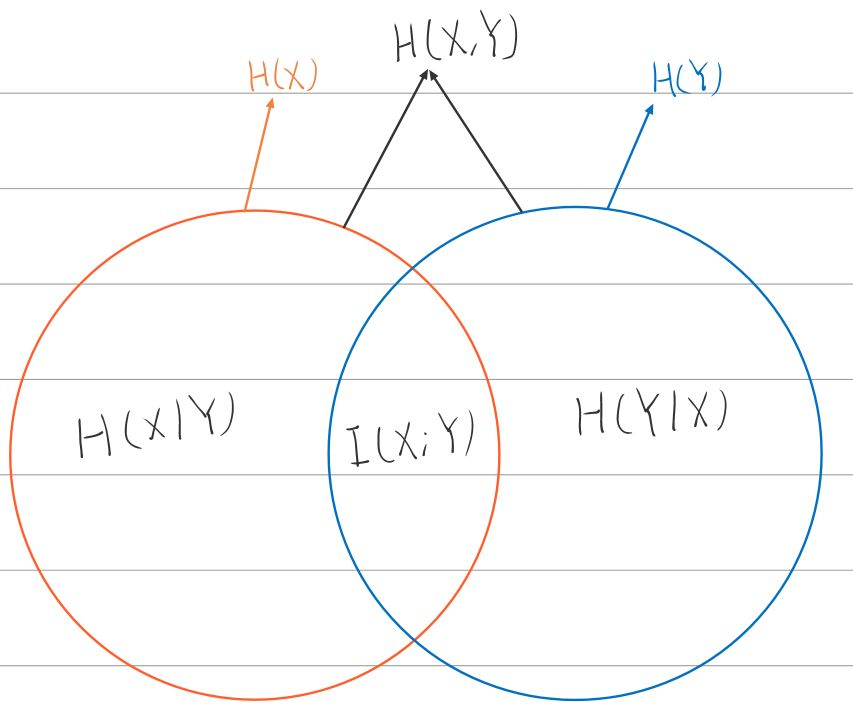
\includegraphics[scale=0.3]{Venn_Diagram}
            \label{fig:figure1}
            \end{figure}
    \item[Problem 4] Solutions:\\
     $H(p(x))=1.5$ bits,\quad $H(q(x))=1.585$ bits.\\[8pt]
     $D[p(x)||q(x)]=\displaystyle\sum_{x\in X}p(x)\log \big[\dfrac{p(x)}{q(x)}\big]=0.085$ bits, $D[q(x)||p(x)]=\displaystyle\sum_{x\in X}q(x)\log \big[\dfrac{p(x)}{q(x)}\big]=0.082$ bits.\\[8pt]So $D[p(x)||q(x)]\neq D[q(x)||p(x)]$.
    \item[Problem 5] Solutions:
        \subitem(a) $H(X)=\displaystyle\sum_{i=1}^{8}p_i(x)\log p_i(x)=2$ bits.
        \subitem(b) $1024\times 3=3072$ bits.
        \subitem(c) $T_{c_2}=\displaystyle\sum_{i=A}^{H}S_{i}N_i=2051$ bits, of which $S_i$ denotes for bits required to send symbol i, while $N_i$ denotes for number of symbol i.
        The average bits used to transmit one symbol is $\dfrac{2051}{1024}=2.0$ bits.
    \item[Problem 6] Solutions:
        \subitem(a) $\rho=\dfrac{H(X_1)-H(X_2|X_1)}{H(X_1)}=\dfrac{I(X_1;X_2)}{H(X_1)}$.
        \subitem(b) As we know,$I(X_1;X_2)\geq 0$ and $I(X_1;X_2)\leq \min(H(X_1),H(X_2))$. So $0\leq \rho \leq 1$.
        \subitem(c) $\rho = 0\Leftrightarrow I(X_1;X_2)=0\Leftrightarrow X_1$ and$X_2$ are independent.
        \subitem(d) $\rho = 1\Leftrightarrow I(X_1;X_2)=H(X_1)\Leftrightarrow H(X_1)-H(X_1|X_2)=H(X_1)\Leftrightarrow X_1=X_2$.
    \item[Problem 7] Solutions:
        \subitem(a) By chain rules, $H(X,Y|Z)=H(X|Z)+H(Y|X,Z)\geq H(X|Z)$, and $Y$ is independent of $X$ given $Z$ for equality.
        \subitem(b) By chain rules, $I(X,Y;Z)=H(X)-H(X|Y,Z)$ and $I(X;Z)=H(X)-H(X|Z)$, $H(X,Y|Z)\geq H(X|Z)$, So $I(X,Y;Z)>I(X:Z)$.The equality condition is the same as last problem.
        \subitem(c) $H(X,Y,Z)-H(X,Y)=H(Z|X,Y)$,$H(X,Z)-H(X)=H(Z|X)$, as $H(Z|X,Y)\leq H(Z|X)$, $H(X,Y,Z)-H(X,Y)\leq H(X,Z)-H(X)$. The equality condition is $X=Y$.
        \subitem(d)\[\begin{aligned}
                          Right&=I(Z;Y|X)-I(Z;Y)+I(X;Z)\\&=H(Z|X)-H(Z|X,Y)-(H(Z)-H(Z|Y))+(H(Z)-H(Z|X))\\&=H(Z|Y)-H(Z|X,Y)\\&=I(Z;X|Y)
                    \end{aligned}\]
                Obviously, $Right=Left$, so the inequality is actually an equality.
\end{description}


\end{document}
